\documentclass[preview,12pt]{article}
\usepackage{amsmath}
\usepackage{gensymb}
\usepackage{ragged2e}
\usepackage{geometry}
\usepackage{graphicx}
\usepackage{caption}
\usepackage{subcaption}
\usepackage{pdfpages}

\geometry{letterpaper, margin=1in}

\begin{document}

\noindent Compressible Flow and Thermodynamics\newline
Josh Coffey \newline
Assignment 2 \newline
9/17/2020 \newline

\section*{1)}
    The rate of heat transfer to the surroundings from a person at rest is about 400 kJ/h. Suppose that the ventilation system fails in an auditorium containing 533 people.
    \subsection*{(a)}
        How much does the internal energy of the air in the auditorium increase during the first 30 minutes after the ventilation system fails? \newline
        Assuming that the auditorium is the system, 
        $$\dot{Q}_{person \rightarrow room}=400\textrm{ }kJ/h$$
        $$\dot{Q}_{tot}=400*533=213,200\textrm{ }kJ/h$$
        30 minutes after the ventilation system fails, the additional heat in the auditorium will be 106,600 kJ.
        \newline
        Know that 
        $$\partial Q =dU+dKE+dPE+\partial W$$
        Because no change in velocity or height of the system (auditorium), $dPE=dKE=0$.
        $$Q=U_2-U_1+W$$
        Assuming the work done to maintain the ventilation system is enough to keep the system in equilibrium, then the rate of work is also -213,200 kJ/h.  However, once the ventilation system fails, then the work being done on the system is 0.  So the above equation becomes
        $$106,600kJ=U_2-U_1$$
        Which is the amount the internal energy of the air increases after 30 minutes of no ventilation system.
    \subsection*{(b)}
        Considering the auditorium and all the people as a system, and assuming no heat transfer to the surroundings, how much does the internal energy of the system change? How do you explain the fact that the temperature of the air increases?
        $$$$
        When you consider the case where the auditorium and the people are the system, then the internal energy of the system will not change.  However, the internal energy of the air will increase as heat transfers from people to the air as shown in part (a).  This explains the increased air temperature.
        
\section*{2)}
One-tenth pound-mass of oxygen is contained in a cylinder fitted with a piston. The initial conditions are 20 lbf/in$^2$, 70$\degree$F. Weights are then added to the piston, and the oxygen is slowly compressed isothermally until the final pressure is 65 lbf/in$^2$ Calculate the work done during this process.

    \begin{center}
    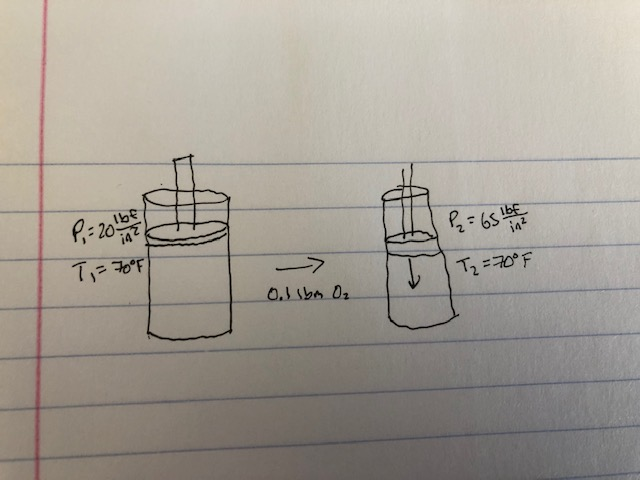
\includegraphics[width=.75\textwidth, angle =90 ]{Problem 2.jpg}
    \end{center}
    Using the polytropic work equation where n=1 and assuming that the $O_2$ is a perfect gas:
    $$W=p_1V_1ln(\frac{V_2}{V_1})=p_1\frac{mRT_1}{p_1}ln\left(\frac{\frac{mRT_2}{p_2}}{\frac{mRT_1}{p_1}}\right)$$
    Since this is an isothermal process:
    $$W=mRTln\left(\frac{p_1}{p_2}\right)=(0.1lbm)\left(\frac{1545.4\frac{ft* lbf}{R*lbmol}}{32lbm/lbmol}\right)(529.67 R)ln(20/65)$$
    $$W=-3014.97ft*lbf$$
    Work is negative in this case because it is being done on the system.
    
\section*{3)}
    Use T-s, p-T and p-v diagrams to plot the possible states between 0.1 and 20 atm that can be reached via an isentropic process from: 
    
    \subsection*{a)}
        Standard day conditions
        $$$$
        Treating air as a perfect gas, can get the temperature at each pressure using the points chosen between 0.1 and 20 atm and the recorded density of air at sea level as values in the equation $p=\rho RT$.  Then can use equation $P_1V_1^n=P_2V_2^n$ to get volume, assuming that $V_1$ is set to be $1m^3$ for a $P_1$=0.1 atm.  Because this process will be isentropic, $n=\gamma=1.4$.  This results in:
        
        \begin{center}
        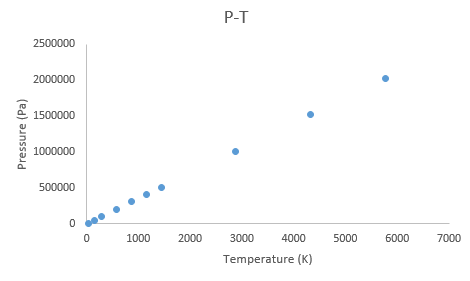
\includegraphics[width=.5\textwidth]{HW2_PT1.PNG}
        \end{center}
        \begin{center}
        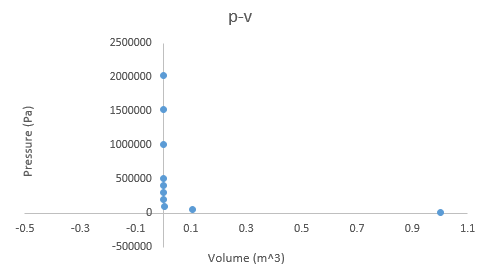
\includegraphics[width=.5\textwidth]{HW2_pv1.PNG}
        \end{center}
        \begin{center}
        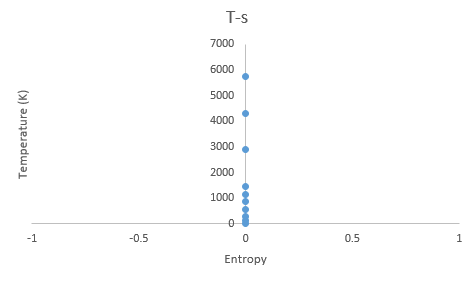
\includegraphics[width=.5\textwidth]{HW2_ts1.PNG}
        \end{center}
    
        As can be seen, the P-T and T-s graphs are linear while p-v is not.
    
    \subsection*{b)}
        Standard atmosphere conditions at 30k ft. 
        $$$$
        Repeating the process in part a but with a new density of air at 30,000 feet gives:
        
        \begin{center}
        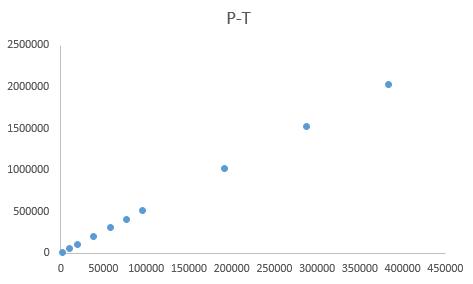
\includegraphics[width=.5\textwidth]{HW2_PT2.PNG}
        \end{center}
        \begin{center}
        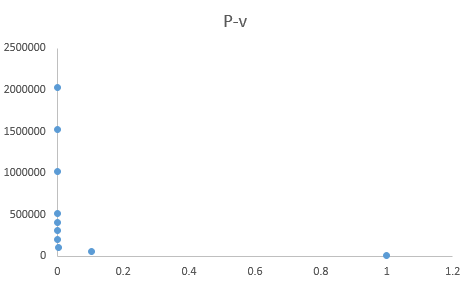
\includegraphics[width=.5\textwidth]{HW2_pv2.PNG}
        \end{center}
        \begin{center}
        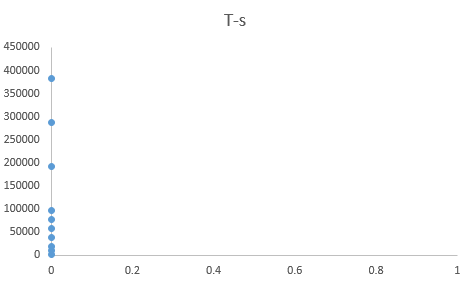
\includegraphics[width=.5\textwidth]{HW2_ts2.PNG}
        \end{center}        
        
        
\section*{4)}
    Starting from the 1st and 2nd Law of thermodynamics between a given state and a fictious stagnation state, derive Shapiro equations 4.14a, b, and c. Be sure to list the particular assumptions made on the process for each equation.
    
    $$\frac{T_0}{T}=1+\frac{k-1}{2}M^2$$
    $$\frac{p_0}{p}=\left(1+\frac{k-1}{2}M^2\right)^\frac{k}{k-1}$$
    $$\frac{\rho_0}{\rho}=\left(1+\frac{k-1}{2}M^2\right)^\frac{1}{k-1}$$
    
    Assuming a the gas is perfect and starting with equation (2.7-1):
    $$ds=c_p\frac{dT}{T}-R\frac{dp}{p}$$
    For isentropic processes, ds=0:
    $$c_p\frac{dT}{T}=R\frac{dp}{p}$$
    Because gas is perfect, can use equation of state $p=\rho R T$:
    $$\frac{c_pdT}{T}=R\frac{dp}{\rho R T}$$
    $$c_p dT=d\frac{p}{\rho}$$
    Using equation of state again:
    $$c_pd(\frac{p}{R\rho})=\frac{dp}{\rho}$$
    Can pull out out R since a constant:
    $$\frac{c_p}{R}d(\frac{p}{\rho})=\frac{dp}{\rho}$$
    Using the quotient rule to differentiate gives:
    $$\frac{c_p}{R}\frac{\frac{dp}{\rho}-pd\rho}{\rho^2}=\frac{dp}{\rho}$$
    $$\frac{c_p}{R}dp-\frac{c_p}{R}p\frac{d\rho}{\rho}=dp$$
    $$\frac{c_p}{R}\frac{dp}{p}-\frac{c_p}{R}\frac{d\rho}{\rho}=\frac{dp}{p}$$
    $$(\frac{c_p}{R}-1)\frac{dp}{p}=\frac{c_p}{R}\frac{d\rho}{\rho}$$
    Using equation 2.5-15:
    $$((\frac{\gamma}{\gamma-1})-1)\frac{dp}{p}=(\frac{\gamma}{\gamma-1})\frac{d\rho}{\rho}$$
    $$\frac{dp}{p}=\gamma\frac{d\rho}{\rho}$$
    Integrating both sides gives:
    $$ln(p)+C=\gamma ln(\rho)+C$$
    $$p=\rho^\gamma+C$$
    $$\frac{p}{\rho^\gamma}=C$$
    Assuming this constant is the total pressure and total density (i.e. the pressure/density when the flow is brought to a stop):
    $$\frac{p_t}{\rho_t^\gamma}=\frac{p}{\rho^\gamma}$$
    Rearranging:
    $$\frac{p}{p_t}=\frac{\rho}{\rho_t}^\gamma$$
    Can use equation of state to get total temperature:
    $$\frac{R\rho T}{R\rho_tT_t}=\frac{\rho}{\rho_t}^\gamma$$
    $$\frac{T}{T_t}=\frac{\rho}{\rho_t}^{\gamma-1}$$
    Using both pressure and temperature equations:
    $$\frac{p}{p_t}=\left(\frac{T}{T_t}\right)^{\frac{\gamma}{\gamma-1}}$$
    Using the equation for enthalpy 3.5-11 in the conservation of energy equation:
    $$h_t=h+\frac{v^2}{2}$$
    $$h_t=c_pT+\frac{v^2}{2}$$
    Know that $v=Mc$, so:
    $$h_t=c_pT+\frac{M^2c^2}{2}$$
    Rewriting to only have $T$
    $$c_pT_t=c_pT+\frac{M^2c^2}{2}$$
    Using the equation for the speed of sound:
    $$c_pT_t=c_pT+\frac{M^2\gamma RT}{2}$$
    $$\frac{T_t}{T}=1+\frac{M^2\gamma R}{2c_p}$$
    From equation 2.5-15:
    $$\frac{T_t}{T}=1+\frac{\gamma}{2}\frac{\gamma-1}{\gamma}M^2=\boxed{1+\frac{\gamma-1}{2}M^2}$$
    Saw above that:
    $$\frac{p}{p_t}=\left(\frac{T}{T_t}\right)^{\frac{\gamma}{\gamma-1}}\implies\frac{p_t}{p}=\boxed{\left(1+\frac{\gamma-1}{2}M^2\right)^\frac{\gamma}{\gamma-1}}$$
    $$\frac{T}{T_t}=\frac{\rho}{\rho_t}^{\gamma-1}\implies \frac{T_t}{T}=\frac{\rho_t}{\rho}^\frac{1}{\gamma-1}\implies\frac{\rho_t}{\rho}=\boxed{\left(1+\frac{\gamma-1}{2}M^2\right)^\frac{1}{\gamma-1}}$$
    
    

\end{document}